\section{Problem (9)}
	\begin{figure}[H]
		\begin{center}
			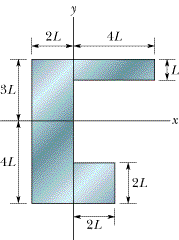
\includegraphics[scale=1]{hw9_problem9}
			\caption{Illustration of Problem 9}
			\label{fig:hw9_problem9}
		\end{center}
	\end{figure}

	\subsection{Question (a)}

		What is the $x$ coordinate of the center of mass for the uniform plate shown in the figure if $L = \ 5.0 \ inches$?

		\textbf{R:}

		\begin{align}
			m_{1} = \ &6L^{2}& \notag \\
			x_{1} = \ &-1L& \notag \\
			m_{2} = \ &4L^{2}& \notag \\
			x_{2} = \ &2L& \notag \\
			m_{3} = \ &4L^{2}& \notag \\
			x_{3} = \ &1L& \notag \\
			m_{4} = \ &8L^{2}& \notag \\
			x_{4} = \ &-1L& \notag \\
			X_{cm} = \ &\frac{(6L^{2})(-1L) + (4L^{2})(2L) + (4L^{2})(1L) + (8L^{2})(-1L)}{6L^{2} + 4L^{2} + 4L^{2} + 8L^{2}}& \notag \\
			= \ &\frac{-2 L^{3}}{22 L^{2}} = \frac{-1}{11}L = \frac{-5 \ in}{11}& \notag \\
			= \ &- 0.\overline{45} \ in&
		\end{align}

	\subsection{Question (a)}

		What is the $y$ coordinate of the center of mass for the uniform plate shown in the figure if $L = \ 5.0 \ inches$?

		\textbf{R:}

		\begin{align}
			y_{1} = \ &1.5L& \notag \\
			y_{2} = \ &2.5L& \notag \\
			y_{3} = \ &-3L& \notag \\
			y_{4} = \ &-2L& \notag \\
			Y_{cm} = \ &\frac{(6L^{2})(1.5L) + (4L^{2})(2.5L) + (4L^{2})(-3L) + (8L^{2})(-2L)}{22L^{2}}& \notag \\
			= \ &\frac{-9L^{3}}{22L^{2}} = \frac{-9}{22}L = \frac{- 45 \ in}{22}& \notag \\
			= \ &- 2.0\overline{45} \ in&
		\end{align}
